\documentclass[letterpaper, 10 pt, conference]{ieeeconf}


\usepackage[colorlinks=true, urlcolor=blue, pdfborder={0 0 0}]{hyperref}
\usepackage{xcolor}
\usepackage{geometry}
\usepackage{overpic}
\usepackage{fancyhdr}
\graphicspath{{./pictures/pdf/},{./pictures/ps/},{./pictures/png/},{./pictures/jpg/}}
\begin{document}
\author{Professor Aaron T. Becker}
\title{How to \emph{join} the Robotic Swarm Control Lab}
\maketitle
\thispagestyle{fancy}
\pagestyle{fancy}
\addtolength{\headsep}{0.2in}
\addtolength{\topmargin}{-0.2in}
\lhead{\small pdf at \href{https://github.com/aabecker/RoboticSwarmControlLab/tree/master/JoiningTheLab}{github.com/aabecker/RoboticSwarmControlLab/}}

\begin{abstract}
The Robotic Swarm Control Lab (RSCL) exists to
 (1) understand, quantify, and implement the best methods for controlling huge numbers of robots, 
 (2)  implement robotic solutions to medical problems, 
 (3)  train confident, productive, ethical engineers to perform impactful research.

This document explains how to earn lab access and the software suite we use.
\end{abstract}

\section{Preliminaries}

We are glad you are interested in the lab and looking forward to getting to know you!  Figure \ref{fig:flowchart} describes the process of joining the lab. First learn about our lab, then level up by completing a literature review and safety training.


\subsection{Learn about our lab}

\begin{enumerate}
\item Browse through 
 our YouTube channel \href{www.youtube.com/aabecker5/}{youtube.com/aabecker5/}, 	\href{http://demonstrations.wolfram.com/author.html?author=Aaron+Becker}{Mathematica Demonstrations}
Gamification research: \href{www.SwarmControl.net}{SwarmControl.net}, 
and papers: \href{scholar.google.com/citations?user=6kGt1DEAAAAJ}{scholar.google.com/Aaron T Becker}.
Decide: Do any of these seem interesting to you? 
	If so, do you have any tools or techniques that could be applied to these?  
	Could you optimize something?
	Do you already have a project you want to pursue?  
	If so, can you show how it aligns with my lab's goals or interests?
\item	Email Prof. Becker.  include your CV, 
	 potential project, 
	why you want to attack this problem,
	any \href{https://docs.google.com/forms/d/1mLb5raedYWEPgWf-Fb2H9JnsHo4Yi7R2FQKvxeAf874/viewform?usp=send_form}{skills (Google form)} you could bring to the lab,
	and funding requirements.  Funding MS students is very difficult, funding PhD students is difficult, but there are some opportunities every semester either through my grants or by applying to external sources.
	
\item	Request a meeting with Prof. Becker, or visit during office hours (at least 12 hours after emailing description)
\end{enumerate}

\begin{figure}[h]
\begin{center}
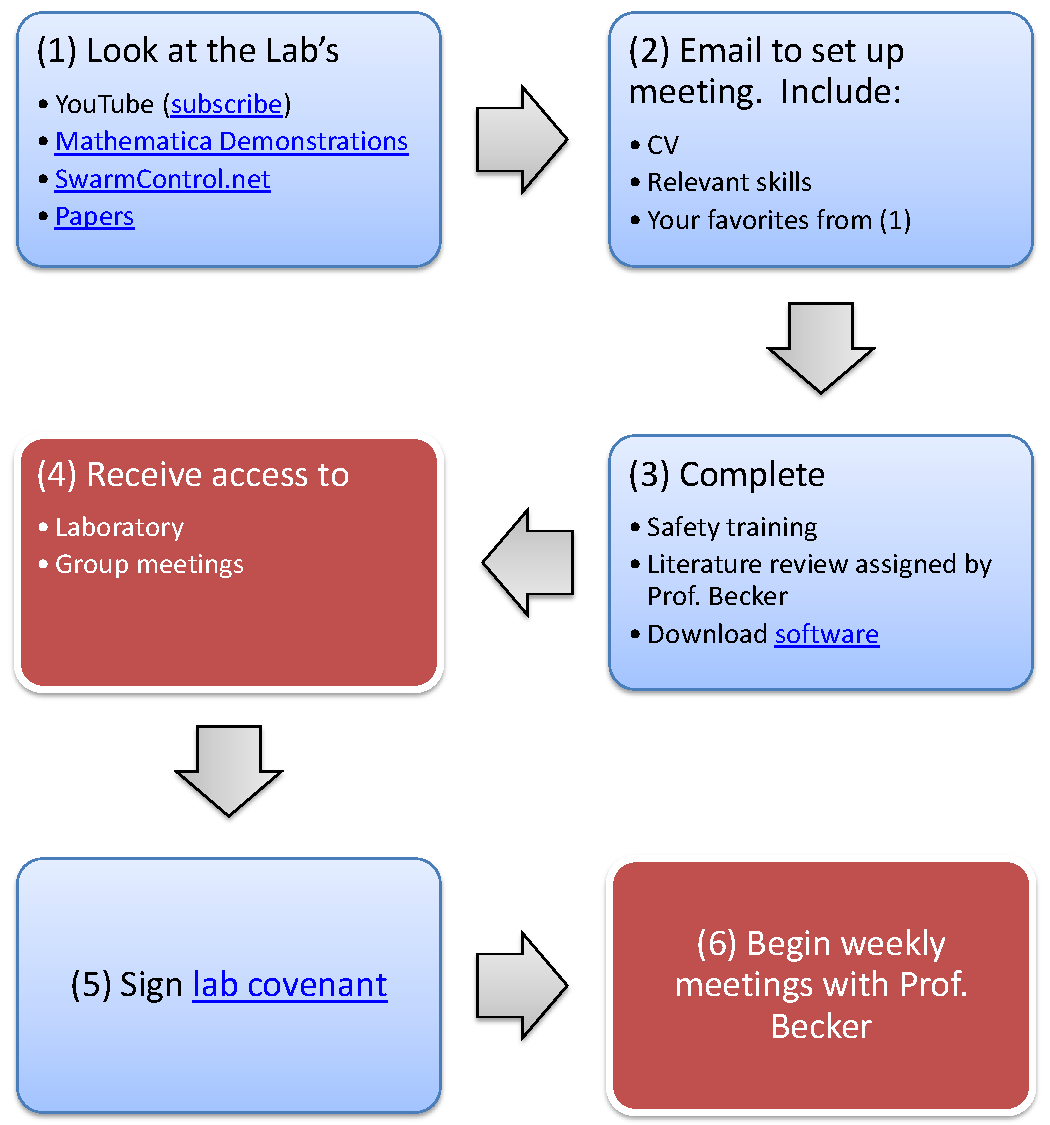
\includegraphics[width=\columnwidth]{JoiningLabFlowChart.pdf}
\caption{Some description of figure.  All plots must have labeled axes with units in parenthesis, for instance:  Robot diameter ($\mu$m)
\label{fig:flowchart}}
\end{center}
\end{figure}

\subsection{Install core software}
Our papers are produced in \href{http://en.wikipedia.org/wiki/LaTeX}{\LaTeX}, a document markup language. \LaTeX~is widely used for the communication and publication of scientific documents in many fields. We use a distributed revision control system called \href{http://en.wikipedia.org/wiki/Git_(software)}{Git} to backup and share our results.

\emph{The following instructions are aimed toward users with Windows operating system. If you use Linux, we will assume you are competent to find your own software.}


\begin{enumerate}
\item download and run the Basic MiKTeX installer to setup a basic TeX/LaTeX system on your computer \href{http://miktex.org/download}{http://miktex.org}

\item install Texmaker, a front end for \LaTeX, \href{http://www.xm1math.net/texmaker/download.html}{http://www.xm1math.net/texmaker/}

\item install \href{https://github.com/}{github}. We submit our code and written documents through github, which serves as a distributed backup. The  repository for our lab is at  \href{https://github.com/aabecker}{github.com/aabecker}.

\item install \href{http://www.mathworks.com/products/matlab/}{\sc{Matlab}}.  Matlab is useful for plotting, simulating, image processing, etc.  It is provided by the University of Houston at \href{http://www.uh.edu/infotech/php/software/list.php}{Software downloads}.

\item (Optional) install \href{https://inkscape.org/en/}{Inkscape}, a professional \href{http://en.wikipedia.org/wiki/Vector_graphics}{vector graphics} editor.  We save our images as \href{http://en.wikipedia.org/wiki/Scalable_Vector_Graphics}{.svg} files, and generate .pdf images that can be used for posters, papers, and presentations.

\item (Optional) install \href{http://www.wolfram.com/mathematica/}{Mathematica}.  Mathematica is useful for equation manipulation, making interactive demonstrations, and making pretty plots.  It is provided by the University of Houston at \href{http://www.uh.edu/infotech/php/software/list.php}{Software downloads}.
\end{enumerate}
 
\section{Earning Lab Access}
Every potential lab member must complete a literature review and lab safety training before being issued access to the robotics lab.

\subsection{The literature review}
Master and PhD scholars primarily share their research through scholarly writing in academic journals and conferences. Members of the RSCL must have one conference paper to be eligible for a Master's degree. Every paper begins with an outline of the problem, followed by an overview of the current solutions in this area this is called the \emph{literature review}. To join the lab \emph{everyone}, from undergraduates to professors, must complete the following literature review!

On a topic selected by Prof. Becker, select no less than eight references from the proceedings of \href{http://ieeexplore.ieee.org/xpl/conhome.jsp?punumber=1000639}{ICRA}, \href{http://ieeexplore.ieee.org/xpl/conhome.jsp?punumber=1000393}{IROS}, or \href{http://www.roboticsconference.org/}{RSS}\footnote{Some conferences are better than others, and some journals are better than others. ICRA, IROS, and RSS are the flagship conferences in robotics.  ICRA and IROS have $\approx$1,000 papers each year, RSS is more elite with $\approx50$ papers.} Go back no more than five years.  Older papers have usually been superseded by new algorithms or technology. \href{http://scholar.google.com/}{scholar.google.com} will help you, you can easily save the references by clicking the [cite] link under each paper in the search, and then select `Import into BibTeX'.

The goal is a concise, high-level research summary. There should be $\approx$ three papers per column.  For each paper, write only one paragraph.  Answer:

\begin{itemize}
\item Goal of their research 
\item Assumptions (centralized control vs decentralized, perfect sensors vs partial state feedback, simulation or experiments, etc.)
\item Limitations (what did they actually do?)
\end{itemize}


A sample literature review is located at \href{
https://github.com/aabecker/RoboticSwarmControlLab/tree/master/JoiningTheLab/LiteratureReview}{JoiningTheLab/LiteratureReview}.

\subsection{Lab Safety training}
Your safety is important to us!
The class \textbf{EH06: General Laboratory Safety and Hazardous Materials Orientation} is mandatory for all lab members. This class can be signed up for online. It is more fun to complete with a friend.

\begin{itemize} 
%\scriptsize
\item \href{http://www.uh.edu/ehls/training/}{http://www.uh.edu/ehls/training/}
\item \href{http://www.uh.edu/ehls/training/eh06/}{http://www.uh.edu/ehls/training/eh06/}
 \end{itemize}

 
 This class includes toxicology, recognition of hazards, personal protective equipment, understanding MSDS's, proper storage of chemicals, proper disposal of chemicals, fire safety and general safety rules


\section{Conclusion}

After you submit your literature review, meet with Prof. Becker and arrange a meeting.  

Some other things to consider:
\begin{itemize}
\item You can join IEEE \href{www.ieee.org/join}{www.ieee.org/join}.  Feel free to mention my member \# 80569446.
\item 
robotics-worldwide is a weekly update of what is happening in robotics. To subscribe, visit
        \href{http://duerer.usc.edu/mailman/listinfo.cgi/robotics-worldwide}{http://duerer.usc.edu/mailman/listinfo.cgi/robotics-worldwide}
        \item IEEE spectrum has a section on robotics: \href{http://spectrum.ieee.org/robotics}{http://spectrum.ieee.org/robotics}
        \item Robohub is another place for robot updates on robotics:  \href{http://robohub.org/}{robohub.org}
\end{itemize}


%\pagebreak
%
%\section{Survey of useful Robotics skills}\label{sec:skillsform}
%\renewcommand{\MakeTextField}[2]{{\vbox to #2{\vfill\hbox to #1{\hrulefill}}}}
%\begin{Form}
%
%
%\noindent\TextField[name=name,width=5cm,charsize=8pt,bordercolor={0.2 0.2 0.7}]{Name:\hspace*{\fill}}\\
%\TextField[name=email,width=5cm,charsize=8pt,color=black]{Email:\hspace*{\fill}}\\
%Status:\hspace*{\fill} \ChoiceMenu[combo,name=status,width=3cm,charsize=10pt,default=undergrad]{\mbox{}}{volunteer,undergrad,MS,PhD} 
%
%\emph{\scriptsize Mark if you have each skill.  Let me know if there is something you really want to learn
%(TODO: parse the output to auto fill a spreadsheet)}
%
%%\begin{Form}
%%{\small\CheckBox{Check here if you like this form3: }}
%% \end{Form}
%
%
%
%\subsection{Mathematics \& Control}
%\begin{itemize} \renewcommand{\labelitemi}{\CheckBox{\tiny}}
%\item Hidden Markov Models (HMM) 
%\item Nonlinear control design
%\item Numerical Optimization
%\item	PID control design
%\item	\href{http://en.wikipedia.org/wiki/Partially_observable_Markov_decision_process}{POMDP} 
%\item	\href{http://cheng.staff.shef.ac.uk/proofguide/proofguide.pdf}{Proof writing}
%\item	\href{http://planning.cs.uiuc.edu/ch4.pdf}{Quaternions}
%\item	Random Process modeling
%\item	Statistical Analysis
%\end{itemize}
%
%\subsection{Electronics}
%\begin{itemize} \renewcommand{\labelitemi}{\CheckBox{\tiny}}
%\item Antenna design
%\item Battery Design
%\item Circuit layout design/fabrication\\ \TextField[name=layoutSoftware,width=1cm,charsize=7pt,color=black]{(what software)}
%\item Microscopy
%\item Oscilloscope use \TextField[name=oscilloscope,width=1cm,charsize=7pt,color=black]{(what brand?)}
%\item Soldering
%\item Surface mount soldering
%\end{itemize}
%
%\subsection{Fabrication Skills}
%\begin{itemize} \renewcommand{\labelitemi}{\CheckBox{\tiny}}
%\item Carpentry  \TextField[name=carpentry,width=1cm,charsize=7pt,color=black]{(framing/finish?)}
%\item CNC
%\item Have you ever made an electromagnet?
%\item Manual milling
%\item Masonry
%\item Welding \TextField[name=welding,width=2cm,charsize=7pt,color=black]{(what metals)}
%\end{itemize}
%
%\subsection{Software}
%\begin{itemize} \renewcommand{\labelitemi}{\CheckBox{\tiny}}
%\item CAD software  \TextField[name=CAD,width=1cm,charsize=7pt,color=black]{(what software)}
%\item DSP programming \TextField[name=DSP,width=1cm,charsize=7pt,color=black]{(what type?)}
%\item LabVIEW 
%\item Linux
%\item Mathematica
%\item Matlab
%\item MRI pulse sequence design (what type?)
%\item \href{http://playerstage.sourceforge.net/}{Player/stage}
%\item \href{www.ros.org}{Robot Operating System (ROS)}
%\item Microprocessors \TextField[name=microcontroller,width=1cm,charsize=7pt,color=black]{(which one)}
%\item OpenCV
%\item Comsol \TextField[name=Comsol,width=1cm,charsize=7pt,color=black]{(what packages?)}
%\item Finite Element Analysis \TextField[name=FEA,width=1cm,charsize=7pt,color=black]{(what software?)}
%\end{itemize}
%\subsection{Programming Languages (indicate skill level  `N'one, `B�asic, `I'ntermediate, `A'dvanced)}
%\begin{itemize} \renewcommand{\labelitemi}{\CheckBox{\tiny}}
%\item C		\hspace*{\fill}\ChoiceMenu[combo,name=C,width=.5cm,charsize=10pt,default=N]{\mbox{}}{N,B,I,A}
%\item C++	\hspace*{\fill}\ChoiceMenu[combo,name=C++,width=.5cm,charsize=10pt,default=N]{\mbox{}}{N,B,I,A}
%\item Java 	\hspace*{\fill}\ChoiceMenu[combo,name=Java,width=.5cm,charsize=10pt,default=N]{\mbox{}}{N,B,I,A}
%\item Python 	\hspace*{\fill}\ChoiceMenu[combo,name=Python,width=.5cm,charsize=10pt,default=N]{\mbox{}}{N,B,I,A}
%\item Ruby on Rails 	\hspace*{\fill}\ChoiceMenu[combo,name=Ruby,width=.5cm,charsize=10pt,default=N]{\mbox{}}{N,B,I,A}
%\item Shell scripting 	\hspace*{\fill}\ChoiceMenu[combo,name=Shell,width=.5cm,charsize=10pt,default=N]{\mbox{}}{N,B,I,A}
%\item Web design 	\hspace*{\fill}\ChoiceMenu[combo,name=WebDesign,width=.5cm,charsize=10pt,default=N]{\mbox{}}{N,B,I,A}
%\item 	\TextField[name=name,width=5cm,charsize=8pt,bordercolor={0.2 0.2 0.7}]{Others:\hspace*{\fill}}
%\end{itemize}
%
%\subsection{Hobbies}
%\begin{itemize} \renewcommand{\labelitemi}{\CheckBox{\tiny}}
%\item Microcontroller programming  (brand?)
%\item Model trains
%\item Quadcopters (construction or piloting?)
%\item RC airplanes (construction or piloting?)
%\item Rocketry
%\end{itemize}
%
%\subsection{Training}
%\begin{itemize} \renewcommand{\labelitemi}{\CheckBox{\tiny}}
%\item Clean room training
%\item IRB training \emph{\small \href{https://www.citiprogram.org/}{at the CITI website} select �Register for the Course�. Select University of Houston as your institution, a username and password, and do coursework for Group 1.}
%\item Machine Shop training
%\item Medical training (CPR, first aid, �)
%\item Travel Planning
%\end{itemize}
%
%\subsection{Fine Arts} \begin{itemize} \renewcommand{\labelitemi}{\CheckBox{\tiny}}
%\item Drawing/Painting/Sculpture   \TextField[name=drawing,width=1cm,charsize=7pt,color=black]{(List:)}
%\item Gardening/cooking/baking \TextField[name=cooking/gardening,width=1cm,charsize=7pt,color=black]{(List:)}
%\item Graphic Design
%\item Music: instrument/sing \TextField[name=music,width=1cm,charsize=7pt,color=black]{(details)}
%\item Photography
%\item Scriptwriting/acting
%\item Sports/Dance/Martial Arts  \TextField[name=sport,width=1cm,charsize=7pt,color=black]{(List:)}
%\item Videography/movie editing  \TextField[name=movie,width=1cm,charsize=7pt,color=black]{(software:)}
%\end{itemize}
%
% \end{Form}
 
 \end{document}